%======================================================================
\section{Sensores}\label{sec:sensores}
%======================================================================
\subsection{Visão geral}

O hub usa três sensores fixos no quarto, e a pulseira usa um sensor inercial e um botão
(Tabela~\ref{tab:sensores}). Todos são módulos comuns e baratos, escolhidos no primeiro
semestre e caracterizados no Projeto 2 daquele semestre; o que mudou desde então foi a faixa
do acelerômetro (Seção~\ref{sec:mpu}) e a forma de ligar cada um à placa nova.

\begin{table}[H]
\centering
\caption{Sensores e interfaces de usuário das duas placas.}
\label{tab:sensores}
\small
\begin{tabular}{@{}>{\raggedright\arraybackslash}p{2.0cm}>{\raggedright\arraybackslash}p{2.4cm}>{\raggedright\arraybackslash}p{2.7cm}>{\raggedright\arraybackslash}p{2.5cm}l>{\raggedright\arraybackslash}p{1.9cm}@{}}
\toprule
Sensor & Mede & Faixa usada & Interface & GPIO & Tensão \\
\midrule
\multicolumn{6}{@{}l}{\textit{Pulseira}} \\
MPU-6050 (módulo GY-521) & aceleração e velocidade angular, 3 eixos & $\pm$8\,g e $\pm$500\,°/s, 16 bits, 200\,Hz & I²C a 400\,kHz + interrupção & 1, 2, 17 & 3,3\,V \\
Botão & ``estou bem'' e pedido de ajuda & --- & digital, \textit{pull-up} interno & 18 & --- \\
\midrule
\multicolumn{6}{@{}l}{\textit{Hub do quarto}} \\
LM35DZ & temperatura do ar & 0 a 57\,°C (limite do ADC) & analógica, 10\,mV/°C, via LM358 & 4 (ADC1) & 5\,V \\
HC-SR501 & movimento de corpos quentes (presença) & até $\sim$7\,m, $\sim$110° & digital, 3,3\,V & 8 & 5\,V \\
MC-38 (até 8) & porta aberta ou fechada & --- & contato seco ao GND & 11, 12 (9, 10) & --- \\
\midrule
\multicolumn{6}{@{}l}{\textit{As duas}} \\
LED WS2812 da DevKit & (atuador) estado e alertas & --- & RMT, 1 fio & 38 ou 48 & 3,3\,V \\
\bottomrule
\end{tabular}
\end{table}

%----------------------------------------------------------------------
\subsection{MPU-6050: acelerômetro e giroscópio}\label{sec:mpu}

O MPU-6050 junta, num mesmo chip MEMS, um acelerômetro e um giroscópio de três eixos, cada
eixo com um conversor de 16 bits, um filtro passa-baixa digital configurável (DLPF) e uma FIFO
de 1024 bytes~\cite{mpu6050}. A comunicação é por I²C. O módulo GY-521 traz um regulador de
3,3\,V e os resistores de \textit{pull-up} do barramento.

\paragraph{Configuração na pulseira.}
\begin{itemize}
  \item \textbf{Faixas:} $\pm$8\,g (4096 contagens por g) e $\pm$500\,°/s (65,5 contagens por °/s).
  \item \textbf{Filtro interno (DLPF):} 44\,Hz no acelerômetro e 42\,Hz no giroscópio. Com ele
        ligado, a taxa interna é de 1\,kHz.
  \item \textbf{Taxa:} 200\,Hz, obtidos dividindo a taxa interna por 5 (\code{SMPLRT\_DIV} = 4).
        Quem marca o tempo é o oscilador do próprio sensor, e não o laço do firmware: no
        primeiro semestre, a amostragem dependia de um \code{vTaskDelay}, e o intervalo
        variava com a carga do processador.
  \item \textbf{Leitura:} cada amostra (6 eixos) ocupa 12 bytes na FIFO. O firmware lê a FIFO a
        cada 50\,ms, ou seja, 10 amostras (120 bytes) por leitura. A FIFO só transbordaria
        depois de $\sim$425\,ms sem leitura, uma folga de mais de oito vezes. O I²C roda a
        400\,kHz, nos GPIOs 1 (SDA) e 2 (SCL); o pino de interrupção vai ao GPIO 17.
  \item \textbf{Consumo:} cerca de 3,9\,mA com os dois sensores ligados~\cite{mpu6050},
        pouco perto do consumo da ESP32-S3 com o rádio ligado.
\end{itemize}

\paragraph{Por que $\pm$8\,g.} No primeiro semestre, o sensor estava em $\pm$2\,g. Os 18
ensaios feitos então (andar, correr e quedas de frente, de costas e de joelhos, com o sensor
na cintura) mostraram o problema (Figura~\ref{fig:mpu_cenarios}): os eixos batem no teto de
2\,g durante a corrida e no impacto das quedas, e a magnitude $\amag$ fica limitada a
$2\sqrt{3} \approx 3{,}46$\,g. Com a saturação, o pico de uma queda e o de um passo de
corrida ficam quase iguais (Figura~\ref{fig:saturacao}); o que sobra para separá-los é a forma
do sinal e o que vem depois do impacto. Em $\pm$8\,g, o teto da magnitude sobe para
$8\sqrt{3} \approx 13{,}9$\,g, e o impacto volta a se destacar da corrida: no exemplo da base
pública SisFall~\cite{sisfall}, 9,0\,g contra 4,7\,g. A perda de resolução não importa:
1/4096\,g por contagem continua abaixo do ruído do sensor.

\begin{figure}[H]
\centering
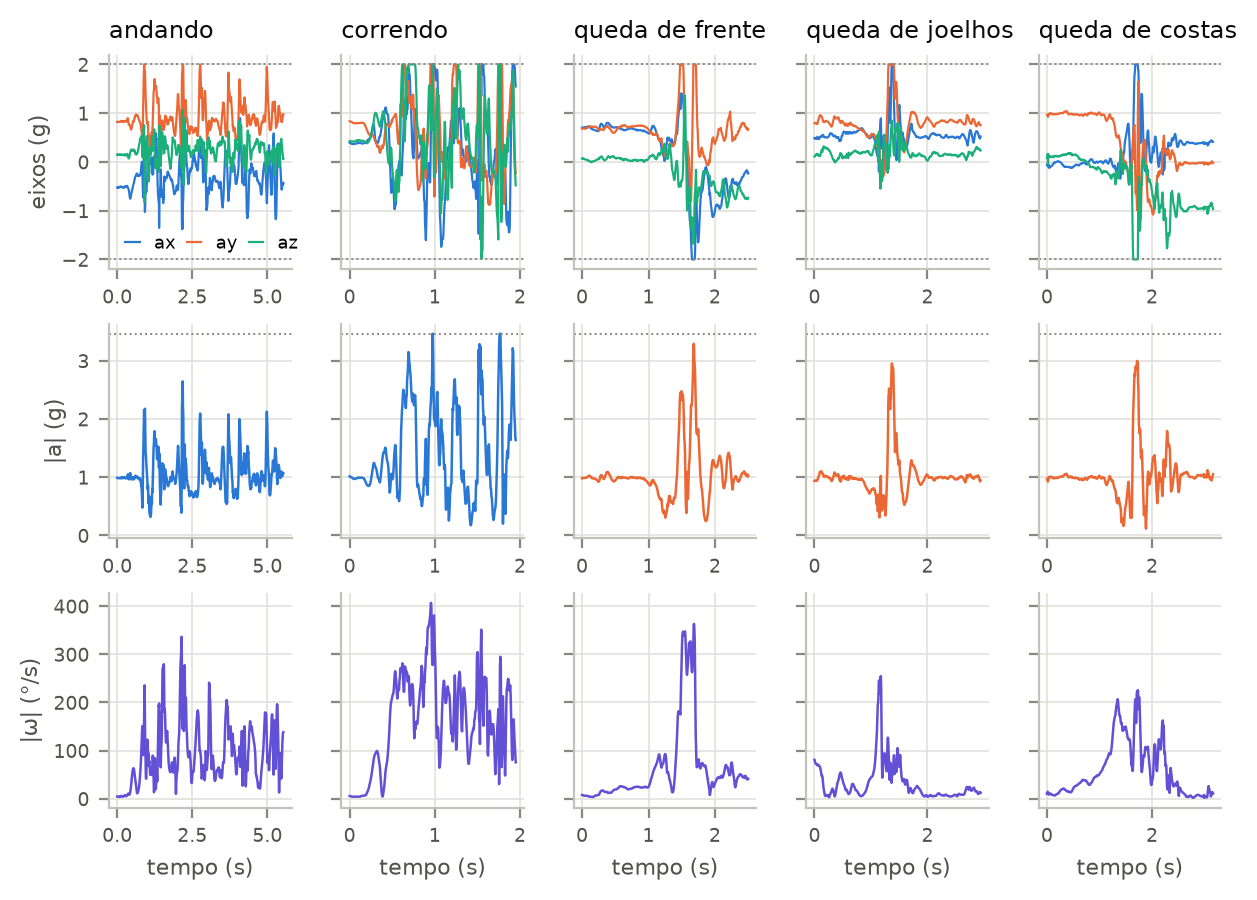
\includegraphics[width=\linewidth]{figuras/fig_mpu_cenarios.png}
\caption{Um ensaio de cada cenário do primeiro semestre (sensor na cintura, $\pm$2\,g):
os três eixos, $\amag$ e $\wmag$. As linhas pontilhadas são o teto de $\pm$2\,g por eixo e o
de 3,46\,g na magnitude. Nas quedas, o padrão é queda livre ($\amag < 1$\,g), impacto e
quietude; na corrida, picos repetidos.}
\label{fig:mpu_cenarios}
\end{figure}

\begin{figure}[H]
\centering
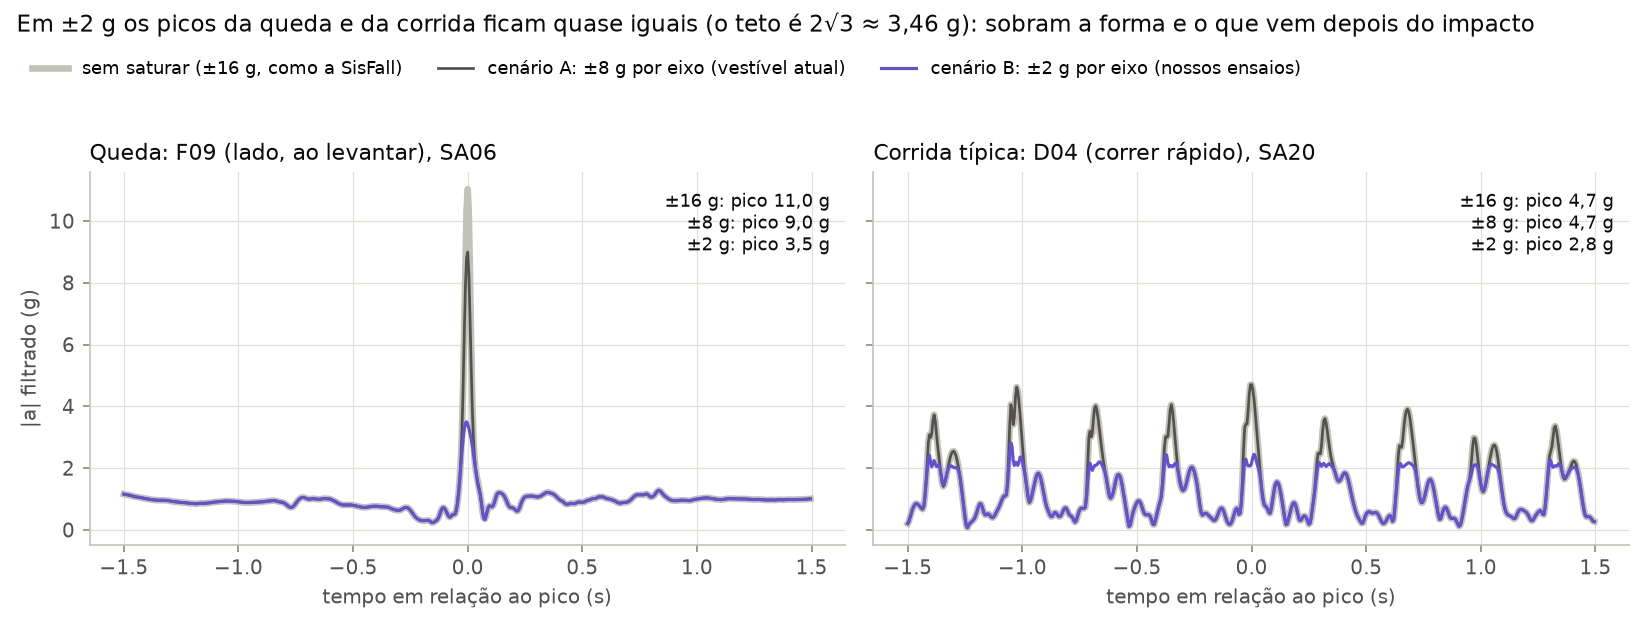
\includegraphics[width=\linewidth]{figuras/fig_saturacao.png}
\caption{Efeito da faixa do sensor em uma queda e uma corrida da SisFall: em $\pm$2\,g, os
dois picos ficam quase iguais. Reproduzida do relatório do Q1~\cite{q1}.}
\label{fig:saturacao}
\end{figure}

%----------------------------------------------------------------------
\subsection{LM35DZ: temperatura}\label{sec:lm35}

O LM35 é um sensor de temperatura integrado com saída em tensão proporcional à
temperatura em Celsius, nominalmente 10\,mV/°C, sem precisar de calibração externa para a
exatidão de catálogo~\cite{lm35}. A versão DZ (encapsulamento TO-92) mede de 0 a 100\,°C,
consome menos de 60\,µA, o que o aquece menos de 0,1\,°C no ar parado, e aceita de 4 a 30\,V.
No hub, ele é alimentado com os 5\,V da placa. A exatidão de catálogo da versão D é a mais
folgada da família (até $\pm$1,5\,°C a 25\,°C); por isso a cadeia inteira foi calibrada contra
uma referência.

\paragraph{Caracterização.} No primeiro semestre, o sensor foi aquecido numa placa
térmica, junto com um termômetro de referência, e dois multímetros leram ao mesmo tempo a
saída do LM35 e a saída do circuito de condicionamento (Figura~\ref{fig:bancada_lm35}). Foram
\lmPontos{} pontos de 0 a 62,2\,°C. O ajuste por mínimos quadrados
(Figura~\ref{fig:lm35}) dá:
\begin{equation}
  V_\text{LM35} = \lmAlfa\,\tfrac{\text{mV}}{\text{°C}}\cdot T + \lmBeta\,\text{mV}
  \qquad (R^2 = \lmRdoisSensor),
\end{equation}
\begin{equation}
  V_\text{cond} = \lmAlfaCadeia\,\tfrac{\text{mV}}{\text{°C}}\cdot T + \lmBetaCadeia\,\text{mV}
  \qquad (R^2 = \lmRdoisCadeia).
  \label{eq:cadeia}
\end{equation}

A inclinação medida no sensor ficou abaixo dos 10\,mV/°C nominais, e os resíduos têm uma
curvatura: o maior desvio é de \lmResMaxCadeia\,°C, no ponto de 0\,°C, e o desvio médio
quadrático na cadeia é de \lmResRmsCadeia\,°C. Como a curva usada no firmware é a da
\emph{cadeia completa} (Eq.~\ref{eq:cadeia}), ela já absorve o ganho real do amplificador e o
desvio do sensor. A razão entre as duas inclinações dá o ganho medido do amplificador,
$\lmAlfaCadeia/\lmAlfa = \lmGanhoMedido$.

\begin{figure}[H]
\centering
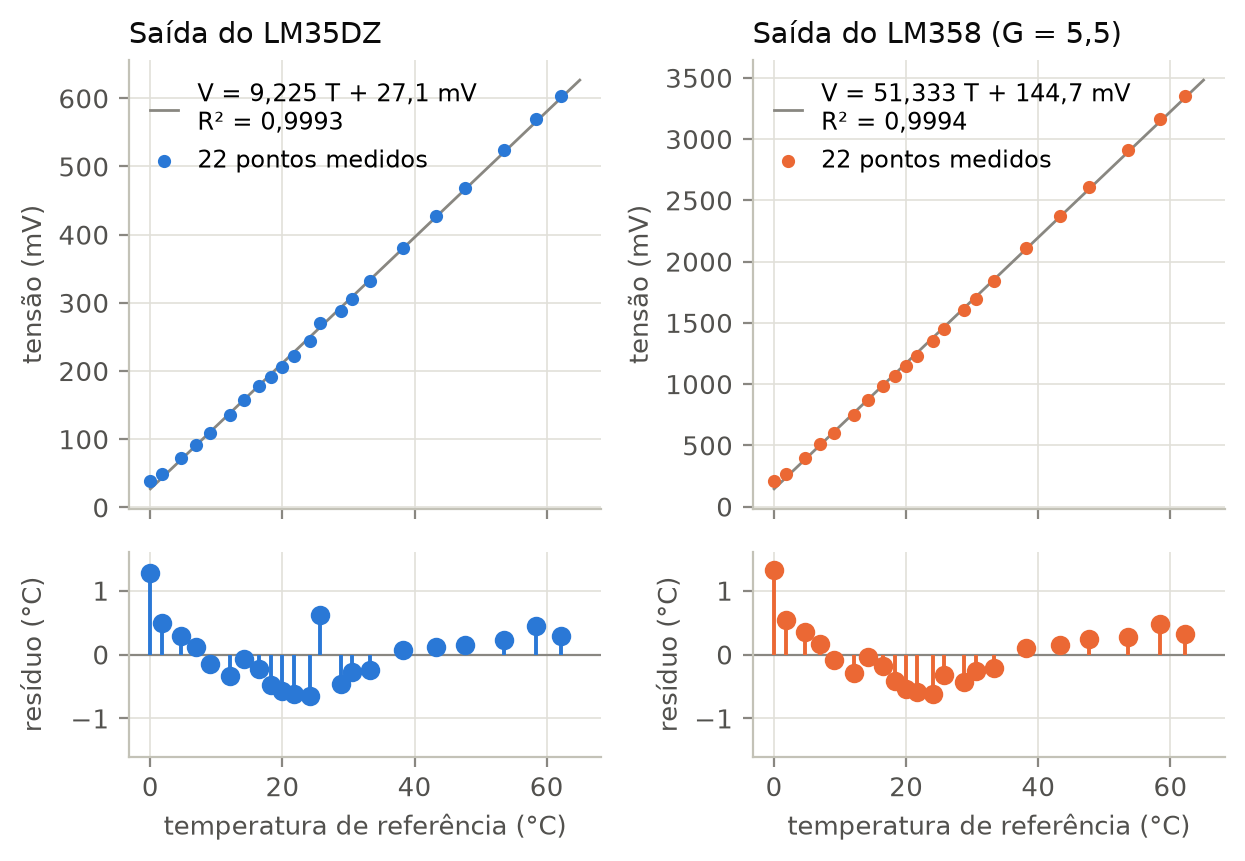
\includegraphics[width=\linewidth]{figuras/fig_lm35_caracterizacao.png}
\caption{Caracterização do LM35DZ: os \lmPontos{} pontos medidos, o ajuste por mínimos
quadrados e os resíduos convertidos em °C. Esquerda: saída do sensor; direita: saída do
condicionamento, que é a curva usada no firmware.}
\label{fig:lm35}
\end{figure}

\begin{figure}[H]
\centering
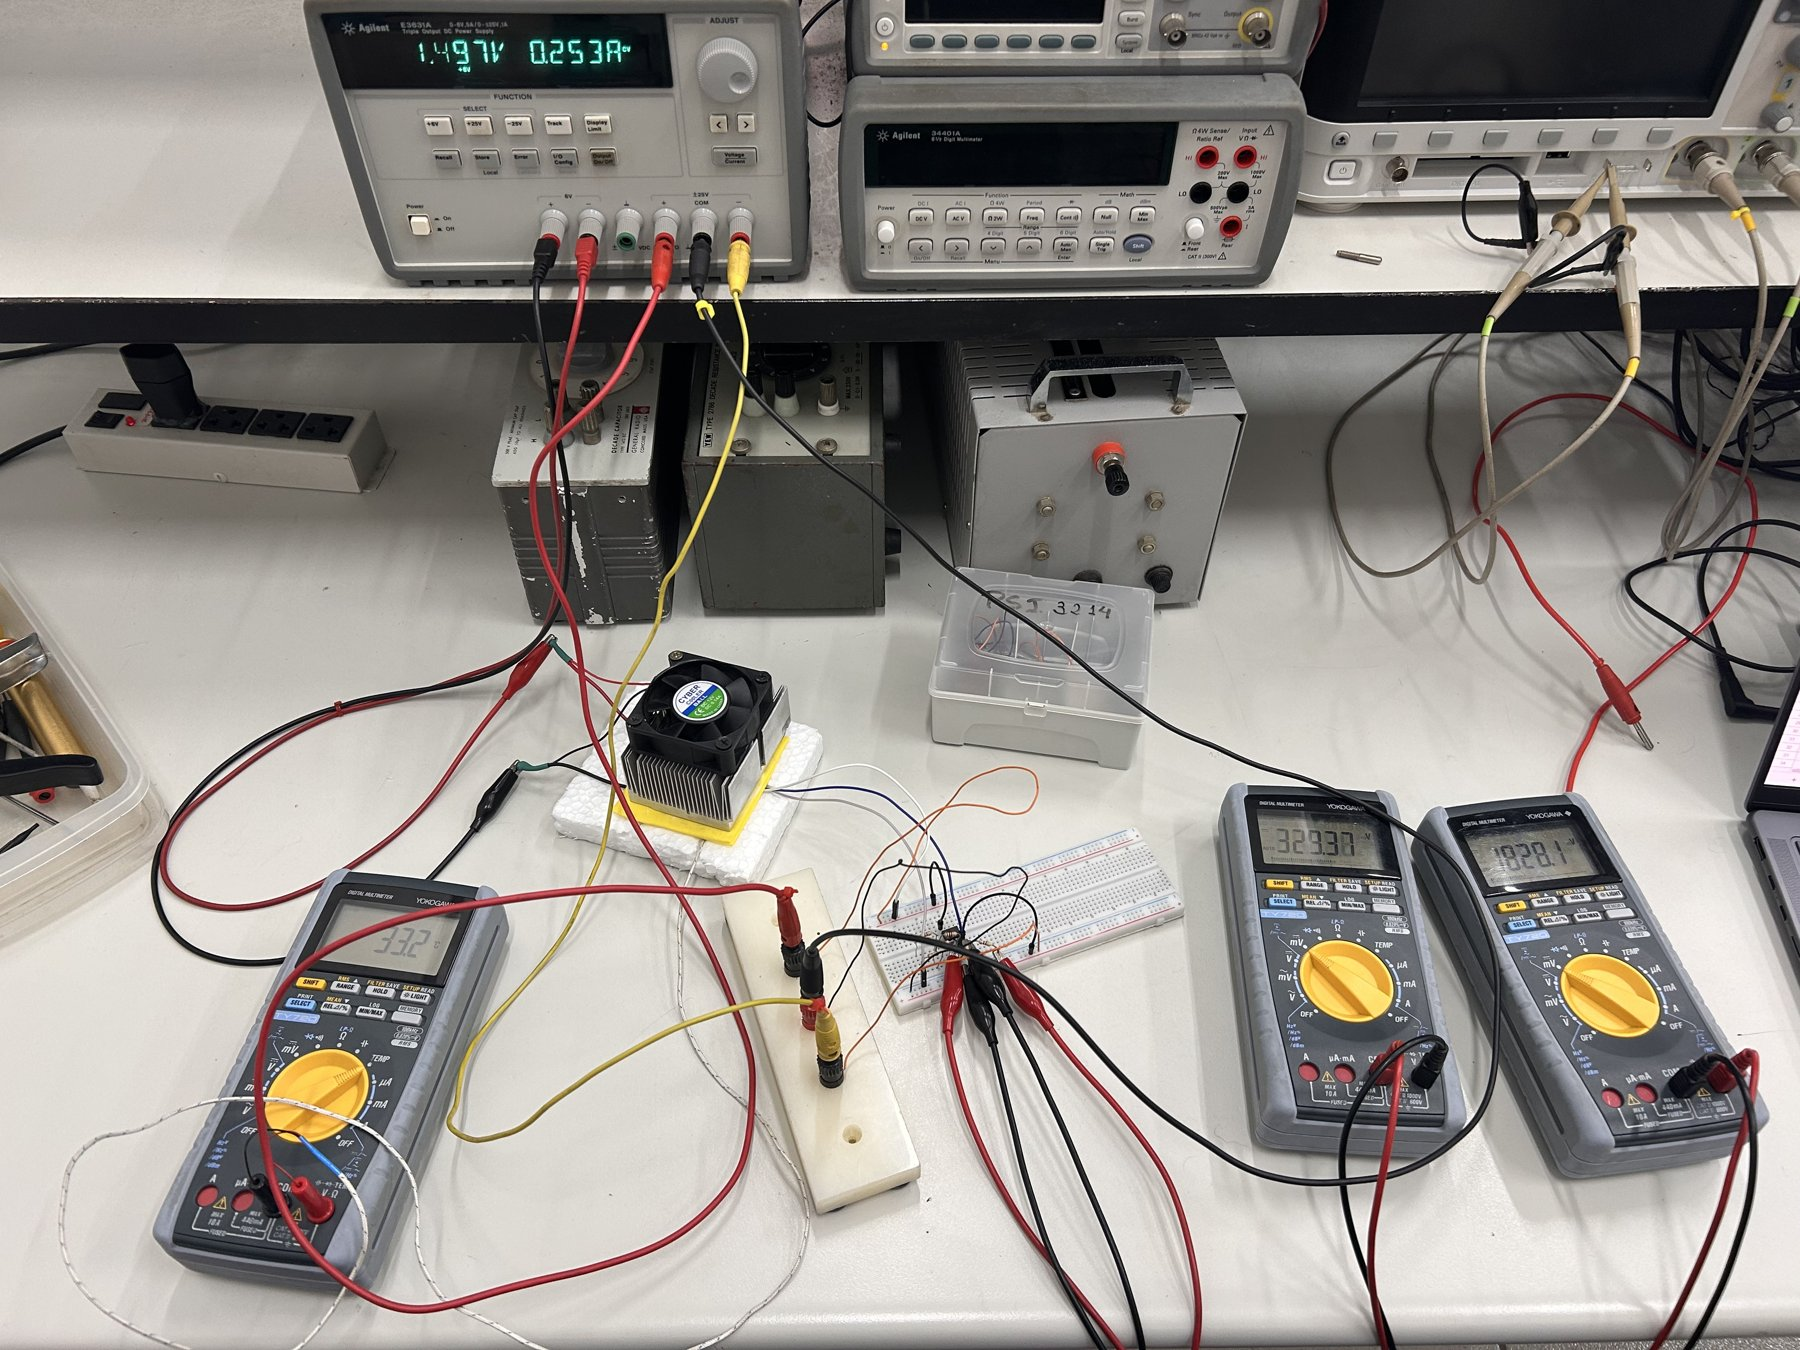
\includegraphics[width=0.78\linewidth]{imagens/s1_bancada_lm35.jpg}
\caption{Bancada da caracterização (primeiro semestre): fonte, placa térmica com o LM35 e
o termômetro de referência, protoboard com o LM358 e os multímetros lendo as duas tensões.}
\label{fig:bancada_lm35}
\end{figure}

%----------------------------------------------------------------------
\subsection{HC-SR501: presença}

O HC-SR501 é um módulo com sensor piroelétrico, lente de Fresnel e um circuito de
tratamento que entrega uma saída digital de 3,3\,V quando detecta o movimento de um corpo
quente~\cite{hcsr501}. Ele vê até cerca de 7\,m, num cone de $\sim$110°, e é alimentado com
5\,V. Dois trimpots ajustam a sensibilidade e o tempo em que a saída fica alta depois da
detecção, e um jumper escolhe o modo; usamos o modo H, em que cada novo movimento renova o
tempo.

Na prática, o sensor vê \emph{movimento}, não presença: uma pessoa dormindo, parada, não o
aciona. É por isso que a regra de inatividade só vale de dia
(Seção~\ref{sec:regras}). O módulo precisa de cerca de um minuto para estabilizar depois de
ligado, e o firmware ignora a saída nos primeiros 60\,s. Ele também tem fama de disparar
sozinho perto do Wi-Fi, o que pesou na posição dele na placa (Seção~\ref{sec:layout}). O
domo precisa sair por um furo na caixa: acrílico e vidro barram o infravermelho.

%----------------------------------------------------------------------
\subsection{MC-38: portas}

O MC-38 é um par reed switch e ímã: com a porta fechada, o ímã fica a poucos
milímetros do reed, e o contato fecha. A ligação é a mais simples possível: um terminal no
GPIO, com o \textit{pull-up} interno da ESP32, e o outro no GND. Porta fechada lê 0; porta
aberta lê 1. Isso tem uma consequência: um fio solto também lê ``aberta'', e não há como
distinguir os dois casos no sinal. Por isso as portas não instaladas são declaradas na
configuração do firmware (Seção~\ref{sec:ausente}).

O contato mecânico \textit{repica} ao fechar, e o fio até a porta funciona como antena. O
tratamento é digital (Seção~\ref{sec:cond_digital}). O hub aceita até 8 portas, uma por
identificador CAN; a placa tem conectores para duas (quarto e banheiro) e GPIOs reservados
para mais seis.

%----------------------------------------------------------------------
\subsection{Botão e LED}\label{sec:botao}

O botão da pulseira (GPIO 18) usa o \textit{pull-up} interno, um capacitor de 100\,nF em
paralelo e o filtro de \textit{glitch} do GPIO. Ele tem dois gestos, e um aperto simples não
faz nada (Tabela~\ref{tab:gestos}):
\begin{itemize}
  \item \textbf{dois toques rápidos} (``estou bem''): cancelam o alerta dos últimos 15\,s, seja
        uma queda, seja um pedido de ajuda. São dois apertos de menos de 1\,s, o segundo
        começando até 1\,s depois de soltar o primeiro;
  \item \textbf{segurar por 3\,s} (``preciso de ajuda''): fora de alerta, abre o alerta
        \code{ajuda}, que segue o mesmo caminho da queda até o cuidador. Cobre a queda que o
        modelo não detectou e qualquer outra situação em que o residente precise de alguém.
\end{itemize}

\begin{table}[H]
\centering
\caption{Gestos do botão da pulseira.}
\label{tab:gestos}
\small
\begin{tabular}{@{}>{\raggedright\arraybackslash}p{4.6cm}>{\raggedright\arraybackslash}p{2.4cm}>{\raggedright\arraybackslash}p{6.8cm}@{}}
\toprule
Estado da pulseira & Gesto & Efeito \\
\midrule
nos 15\,s depois de uma queda ou de um pedido de ajuda (LED vermelho) & dois toques & cancela esse alerta (\code{FALL\_CANCEL} ou \code{HELP\_CANCEL}) \\
normal & segurar 3\,s & pedido de ajuda (\code{HELP}), com a mesma janela de 15\,s para cancelar \\
qualquer um & aperto simples & nada \\
nos 15\,s depois de um alerta & segurar & nada: o alerta já está aberto \\
normal & dois toques & nada: não há alerta para cancelar \\
\bottomrule
\end{tabular}
\end{table}

Os gestos foram escolhidos pelo pior caso de cada um. Quem cai pode ficar deitado sobre o
braço, com o botão apertado pelo corpo; se segurar cancelasse o alerta, a queda real seria
cancelada justamente nessa hora. A pressão do corpo produz um aperto longo, nunca dois toques
separados, e por isso o cancelamento é por dois toques. Para pedir ajuda, segurar é o gesto
comum dos dispositivos de emergência: não exige precisão de tempo, o que importa para quem
tem tremor ou artrite, e uma batida ou um esbarrão não chega a 3\,s. Um pedido feito sem
querer (dormindo sobre o braço, por exemplo) é cancelado pelos mesmos dois toques e, no pior
caso, custa uma visita do cuidador; um cancelamento sem querer deixaria alguém caído sem
socorro. Os tempos são ajustáveis no \code{menuconfig}, para calibrar com os residentes.

O LED é o WS2812 da própria DevKit, controlado pelo periférico RMT. No hub, ele pisca verde a
1\,Hz em operação normal, amarelo sem broker e vermelho a 4\,Hz com um alerta aberto; na
pulseira, pisca vermelho durante os 15\,s em que um alerta pode ser cancelado, e um vermelho
lento indica que o sensor não responde. O buzzer previsto no início foi retirado em outubro:
a sinalização local fica só com o LED, e o alerta chega ao cuidador pela central.
